\documentclass[]{report}
\usepackage[hmargin=1.25in,vmargin=1in]{geometry} %调整页边距
% \usepackage[inner=1in,outer=1.25in]{geometry} %书籍左右不等宽排版
\usepackage[utf8]{inputenc}
\usepackage[]{ctex} %据说可以直接调用诸如 \kaishu \fangsong \heiti 的命令修改字体
\usepackage[svgnames]{xcolor} % Using colors
% \usepackage{background} % To include background images
\usepackage{fancyhdr} % Needed to define custom headers/footers
\usepackage[]{xeCJK}
\setCJKmainfont[BoldFont = STHeiti, ItalicFont = STKaiti]{Songti SC Light} %中文主字体
\setCJKsansfont[BoldFont = Weibei SC, ItalicFont = HanziPen SC]{Xingkai SC Light} %中文无衬线字体
\setCJKmonofont[BoldFont = Libian SC, ItalicFont = STFangsong]{Yuanti SC Light} %中文等宽字体
\setmainfont{Times New Roman} %\rmfamily
\setsansfont[ItalicFont = American Typewriter]{Comic Sans MS} %\sffamily
\setmonofont{Courier} %\ttfamily
\newfontfamily\monaco{Courier} % 用于代码段字体设置
\usepackage{titlesec}
\titleformat{\chapter}{\centering\huge\bfseries}{第~\thechapter~章}{1em}{}
\titleformat{\section}{\Large\bfseries}{第~\thesection~题}{1em}{}
\titleformat{\subsection}{\bfseries}{~}{1em}{}
\usepackage{lipsum} %填充文本

\usepackage{ulem} %解决下划线、删除线之类的
\usepackage{listings}
\lstset{
language=C++,
numberstyle = \monaco,
basicstyle = \monaco,
keywordstyle = \color{blue}\bfseries,
commentstyle=\color[HTML]{006400},
tabsize = 4,
%backgroundcolor=\color{bg}
emph = {int,float,double,char},emphstyle=\color{cyan},
emph = {[2]const, typedef},emphstyle = {[2]\color{red}} }

\makeatletter
\newif\if@restonecol
\makeatother
\let\algorithm\relax
\let\endalgorithm\relax
\usepackage[linesnumbered,ruled,vlined]{algorithm2e}%[ruled,vlined]{
\usepackage{algpseudocode}
\usepackage{amsmath}
\renewcommand{\algorithmicrequire}{\textbf{Input:}}  % Use Input in the format of Algorithm
\renewcommand{\algorithmicensure}{\textbf{Output:}} % Use Output in the format of Algorithm

\usepackage{amsmath} %数学公式问题
\usepackage{amsthm} %公式环境,如proof
\usepackage{booktabs} %三线表
\newcommand{\tabincell}[2]{\begin{tabular}{@{}#1@{}}#2\end{tabular}} %解决单元格内部换行的问题
% 比如这个 Beijing & 0,5 & 1,6 & 2,7 & 3,8 & 4,9 & The number changes every 3 months \\
% 改成这个 \tabincell{l}{Beijing}& \tabincell{c}{0,5}& \tabincell{c}{1,6}& \tabincell{c}{2,7}& \tabincell{c}{3,8}& \tabincell{c}{4,9}& \tabincell{c}{The number changes \\ every 3 months} \\
% 一个单元格过长,整行都需要修改
% 可以配合 \resizebox*{h-width}{v-width}{contents, e.g.tabular} 使用

\usepackage{mathrsfs} %在公式里面使用那个最花的字体
\usepackage{amssymb} %公式里面用空心黑体和旧式字体
\usepackage{amssymb} %AMS符号
\usepackage{amsthm} %AMS定理环境

\usepackage{markdown} %使用markdown语法,在编译时需要打开 shell-escape 标记,即 $ xelatex --shell-escape example.tex
\markdownSetup{hashEnumerators = true} %允许使用 #. 的方式编写有序列表
\markdownSetup{inlineFootnotes = true} %允许使用脚注形式的超链接,调用语法为 [anchor](uri), ^[footnote], <uri>
\markdownSetup{fencedCode = true} %以反引号和缩进来插入代码段,相当于 verbatim
\markdownSetup{
  pipeTables = true
} %支持表格的用法 (图片已经在markdown包里面支持了)
% \usepackage{booktabs} %解决三线表的线条粗细问题

\usepackage{graphicx} %插入图片
\usepackage{pdfpages} %插入PDF文件
\usepackage{makeidx}

\usepackage{tikz} %带圈字符
\usepackage{etoolbox} %带圈字符 (提供robustify)
\usepackage{enumitem}
\newcommand*{\circled}[1]{\lower.7ex\hbox{\tikz\draw (0pt, 0pt)%
    circle (.5em) node {\makebox[1em][c]{\small #1}};}} %新定义命令:带圈字符
\robustify{\circled}
% \usepackage{enumerate} %有序列表

\usepackage{hyperref} %超链接
% \usepackage[hidelinks]{hyperref} %隐藏超链接的红框
\markdownSetup{
  inlineFootnotes = true,
  renderers = {
    link = {\href{#3}{#1}},
  }
} % markdown块中使用直接点进去的超链接
% \setlist[enumerate,1]{label=(\arabic*).,font=\textup,leftmargin=7mm,labelsep=1.5mm,topsep=0mm,itemsep=-0.8mm}
% \setlist[enumerate,2]{label=(\alph*).,font=\textup,leftmargin=7mm,labelsep=1.5mm,topsep=-0.8mm,itemsep=-0.8mm}

\usepackage{braket}

%%%%%% Setting up the style

% \setlength\parindent{0pt} % Gets rid of all indentation
% \backgroundsetup{contents={\includegraphics[width=\textwidth]{ustc-name.pdf}},scale=0.4,placement=top,opacity=0.6,color=cyan,vshift=-20pt} %  USTC Logo

\pagestyle{fancy} % Enables the custom headers/footers

% 使用默认的Chapter页眉
% \lhead{} \rhead{} % Headers - all  empty

% \title{\vspace{-1.8cm}  \color{DarkRed} Laboratory Rotation Report}
% \subtitle{Title of the proposal % Title of the rotation project
% \vspace{-2cm} }
% \date{\today} % No date

\lfoot{\color{Grey} \textit{艾语晨}}  % Write your name here
\rfoot{ \color{Grey} 算法基础 }
\cfoot{\color{Grey} \thepage}

\renewcommand{\headrulewidth}{0.0pt} % No header rule
\renewcommand{\footrulewidth}{0.4pt} % Thin footer rule

\title{{\huge {算法基础第一次作业}}}
\author{艾语晨~PB18000227}
\date{\today}

\linespread{1.3} %行间距为1.3倍默认间距 (1.3 x 1.2倍字符宽度)

\makeindex

\begin{document}
\theoremstyle{definition} \newtheorem{theorem}{Thm}[section] %定义一个定理Thm,序号为section的下一级序号
\theoremstyle{definition} \newtheorem{definition}{Def}[section] %定义一个定义Def,序号为section的下一级序号
\theoremstyle{plain} \newtheorem{lemma}{lemma}[section] %引理

	\maketitle
	\newpage

	\tableofcontents
	\newpage

  \chapter{第二周作业}
    \section{}%第一题
    \begin{figure}[h!]
        \centering
        
\includegraphics[scale=0.3]{images/Pro_1.png}
    \end{figure}
    \subsection{a.}
      假设数组的下标从1开始,伪代码如下:
      \begin{algorithm}
          \caption{Searching in an Array}
          \KwIn{An array $A=\{a_1,\dots,a_n\}$ and the target value $v$}
          \KwOut{$output$,为下标$i$使得$v=A[i]$,或当$v$不在A中出现时,为特殊值$NIL$}
          $output=NIL$\\
          \For{$i=1$\textbf{to}$A.length$}{
            \If{$A[i]==v$}{
              $output=i$
            }
          }
          \If{\textbf{\textrm{not}} $output>0$}{
            $output=NIL$
          }
          \Return{output}
      \end{algorithm}\par
      用循环不变式来证明此算法是正确的:\textit{循环不变式:在循环每一次迭代的开始,包含元素}$A[1..i-1]$\textit{的子数组构成了当前已比较过的元素集合,剩余的子数组}$A[i..n]$\textit{对应于待比较的元素}
      \begin{enumerate}
        \item \textbf{初始化:}在第一次迭代之前(当$i=1$时),已比较过的部分为空,所以该部分是比较过的,而且没有匹配,所以输出为NIL,这表明第一次循环迭代之前循环不变式成立
        \item \textbf{保持:}每一次循环迭代中,都比较第$i$个位置的数组元素,比较之后无论是否匹配都会归入已比较过的部分,并根据比较是否成功修改输出
        \item \textbf{终止:}在循环终止时,由于导致\textbf{for}循环终止的条件是$i>A.length=n$,以及$i$每一次循环加一,故有$i=n+1$。这时所有元素均比较完毕。因此算法正确
      \end{enumerate}\par
    \subsection{b.}
      平均需要检查$\frac{1+\cdots+n}{n}=\frac{n+1}{2}$个元素才可以得到结果,最坏情况是$n$次(当$v=A[n]$时),这两个都是$\Theta(n)$的

    \section{}%第二题
    \begin{figure}[h!]
      \centering
      
\includegraphics[scale=0.3]{images/Pro_2.png}
    \end{figure}
    \subsection{a.}
      不一定。
      \begin{proof}
        如取$f(n)=\frac{1}{n}$,则有$f(n)^2=\frac{1}{n^2}$,又由于$\displaystyle\lim_{n\to\infty}\frac{\frac{1}{n}}{\frac{1}{n^2}}=\infty$,故$\frac{1}{n^2}$不能作为$f(n)$的渐进上界
      \end{proof}
    \subsection{b.}
      正确。
      \begin{proof}
        当$n$足够大时,$\max\{f(n),g(n)\}=O(f(n))=O(g(n))$。不妨设当$n\ge n_0$时,有$\max\{f(n),g(n)\}=f(n)$,且$f(n),g(n)$非负,则可以取$c_1=1,\ c_2=2$,则可以满足$c_1\max\{f(n),g(n)\}=f(n)\le f(n)+g(n)\le 2f(n)=c_2\max\{f(n),g(n)\}$,即证
      \end{proof}
    \subsection{c.}
      正确。
      \begin{proof}
        $O(f(n))$满足对所有$n\ge n_0\ge0$,有$0\le O(f(n))\le f(n)$。当$O(f(n))=f(n)$时,$LHS=2f(n)=\Theta(2f(n))=\Theta(f(n))=RHS$;当$O(f(n))=o(f(n))$时,有$LHS=f(n)+o(f(n))=\Theta(f(n)+o(f(n)))=\Theta(f(n))=RHS$
      \end{proof}
    \subsection{d.}
      错误。
      \begin{proof}
        若$f(n)=\Omega(g(n))$,则对所有$n>n_0$,有$0\le cg(n)\le f(n)$,但$f(n)=o(g(n))$要求对于所有$n>n_0$,有$cg(n)>f(n)\ge0$,故矛盾
      \end{proof}

    \section{}%第三题
    \begin{figure}[h!]
      \centering
      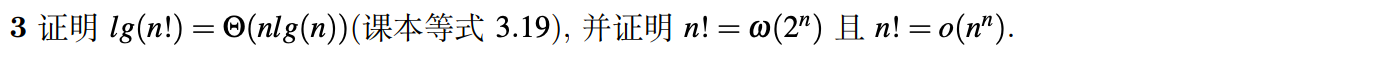
\includegraphics[scale=0.3]{images/Pro_3.png}
      \caption{第三题题目}
    \end{figure}
    \begin{proof}
      由Stirling公式可得:
      \[\begin{aligned}
        \lg(n!)&=\lg\left(\sqrt{2\pi n}\left(\frac{n}{e}\right)^n\left(1+\Theta\left(\frac{1}{n}\right)\right)\right)\\
        &=\frac{1}{2}\lg(2\pi n)+n\lg\left(\frac{n}{e}\right)+\lg\left(1+\Theta\left(\frac{1}{n}\right)\right)\\
        &=\Theta\left(lg(n)+nlg(n)+lg\left(\frac{1}{n}\right)\right)\\
        &=\Theta(nlg(n))
      \end{aligned}
      \]
      \[\lim_{n\to\infty}\frac{n!}{2^n}=\frac{1}{2}\times\frac{2}{2}\times\frac{3}{2}\times\frac{4}{2}\times\frac{5\times6\times\cdots}{2\times2\times\cdots}=\frac{3}{2}\times\frac{5\times6\times\cdots}{2\times2\times\cdots}=\infty
      \]
    \end{proof}

    \section{}%第四题
    \begin{figure}[h]
      \centering
      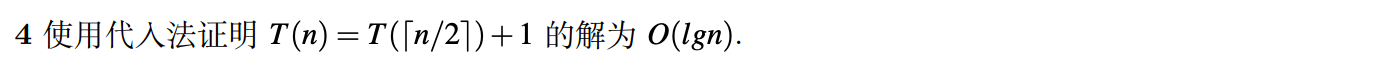
\includegraphics[scale=0.3]{images/Pro_4.png}
    \end{figure}
    \begin{proof}
      假设$T(1)=\Theta(0)=\Theta(\lg1)$。假设当$k<n$时,有$T(k)\le c\lg(k)$,则当$k=n$时,有(取$c\ge1$)
      \[\begin{aligned}
        T(n)&=T(\lceil n/2\rceil)+1\\
        &\le c\lg(\lceil n/2\rceil)+1\\
        &\le c\lg n
      \end{aligned}
      \]需满足$\displaystyle c\ge\frac{1}{\lg(\frac{n}{\lceil n/2\rceil})}$。取$c=\frac{1}{\lg(3/2)}$即可
    \end{proof}\newpage

    \section{}%第五题
    \begin{figure}[h!]
      \centering
      
\includegraphics[scale=0.3]{images/Pro_5.png}
    \end{figure}
    递归树如图所示:
    \begin{figure}[h!]
      \centering
      \includegraphics[scale=0.1]{images/Pro_5_tree.jpg}
      \caption{Recursion Tree}
    \end{figure}\par
    故可以猜想$T(n)=\Theta(n^2)$

    \section{}%第六题
    \begin{figure}[h]
      \centering
      \begin{minipage}{40em}
        \centering
        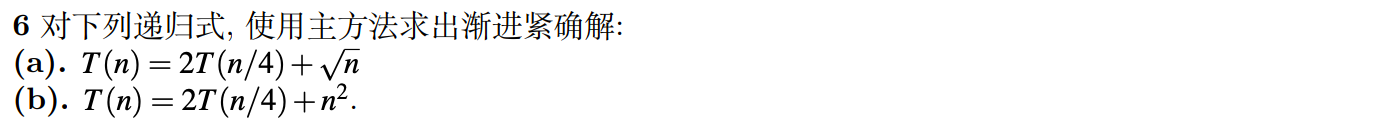
\includegraphics[scale=0.3]{images/Pro_6.png}
      \end{minipage}\\
      \begin{minipage}{40em}
        \centering
        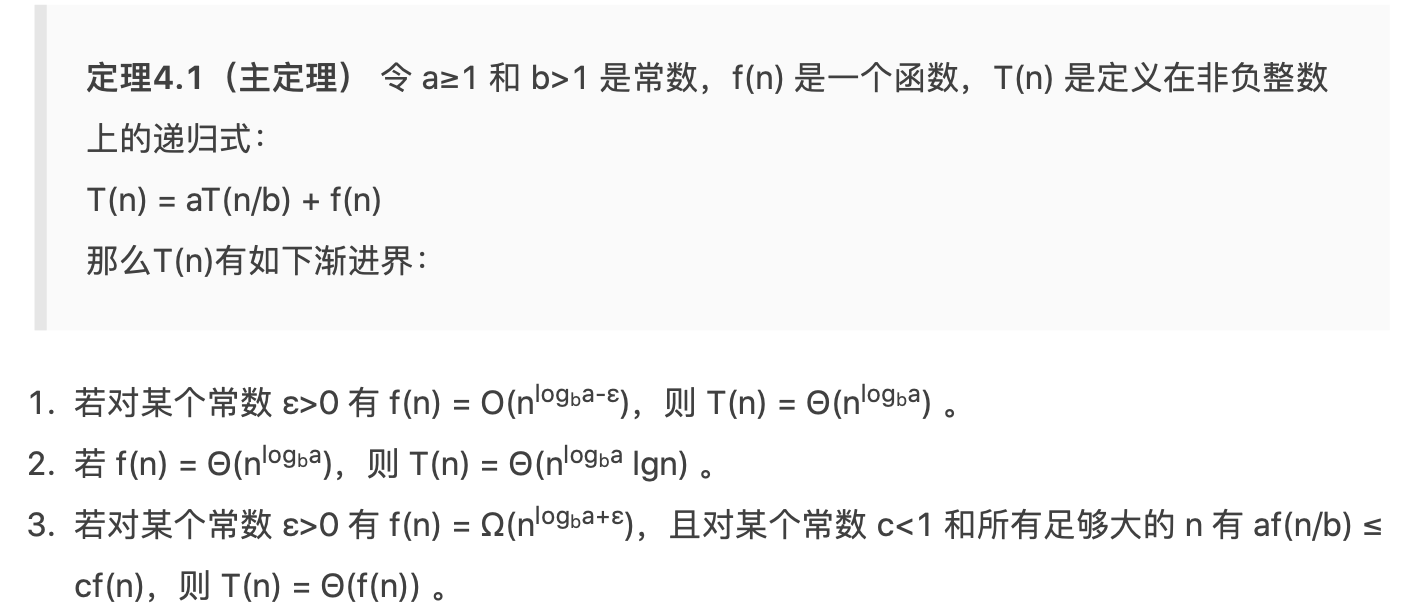
\includegraphics[scale=0.27]{images/Master_Theorem.png}
      \end{minipage}
    \end{figure}
    \subsection{a.}
      对于本题,$a=2,\ b=4\ f(n)=\sqrt{n}$,因此$n^{\log_ba}=\sqrt{n}=\Theta(\sqrt{n})=f(n)$,故$T(n)=\Theta(\sqrt{n}\lg n)$
    \subsection{b.}
      对于本题,$a=2,\ b=4\ f(n)=n^2$,因此$n^{\log_ba}=\sqrt{n}=\Theta(\sqrt{n})=\Omega(n^2)=f(n)$,故$T(n)=\Theta(n^2)$

    \section{}%第七题
    \begin{figure}[h]
      \centering
      
\includegraphics[scale=0.3]{images/Pro_7.png}
    \end{figure}
    不可以应用主方法,因为$a=4,b=2$,故$n^{\log_24=n^2}$。如PPT $topic2\ page64$所言,对于$\forall\varepsilon>0$,有$n^{\varepsilon}=\omega(\lg n)$,故不能在多项式意义下对$f(n)$和$n^2\lg n$进行比较,故不能应用主方法


\end{document}
